%Zarantonello Umberto 21-05-27

\section{Diffusione elettronica per studi subnucleari}
Gli elettroni, come abbiamo già visto precedentemente, sono considerati la sonda principe per l'indagine subnucleare in quanto sono privi di struttura (per quanto ne sappiamo possono essere considerati puntiformi) e interagiscono solamente elettromagneticamente, ovvero tramite una teoria conosciuta con un livello di precisione estremo (probabilmente è attualmente la teoria meglio descritta della fisica).
Conoscendo perfettamente l'interazione tra il nucleone e l'elettrone ci permette di acquisire dettagli sulla struttura del nucleone.

La relazione tra la lunghezza d'onda e la quantità di moto dell'elettrone abbiamo visto che è
\begin{equation}
\lambda\sim \frac{h}{p}
\end{equation}
Introduciamo i grafici di Feynman di un'interazione di questo tipo
\begin{figure}[h]
\centering
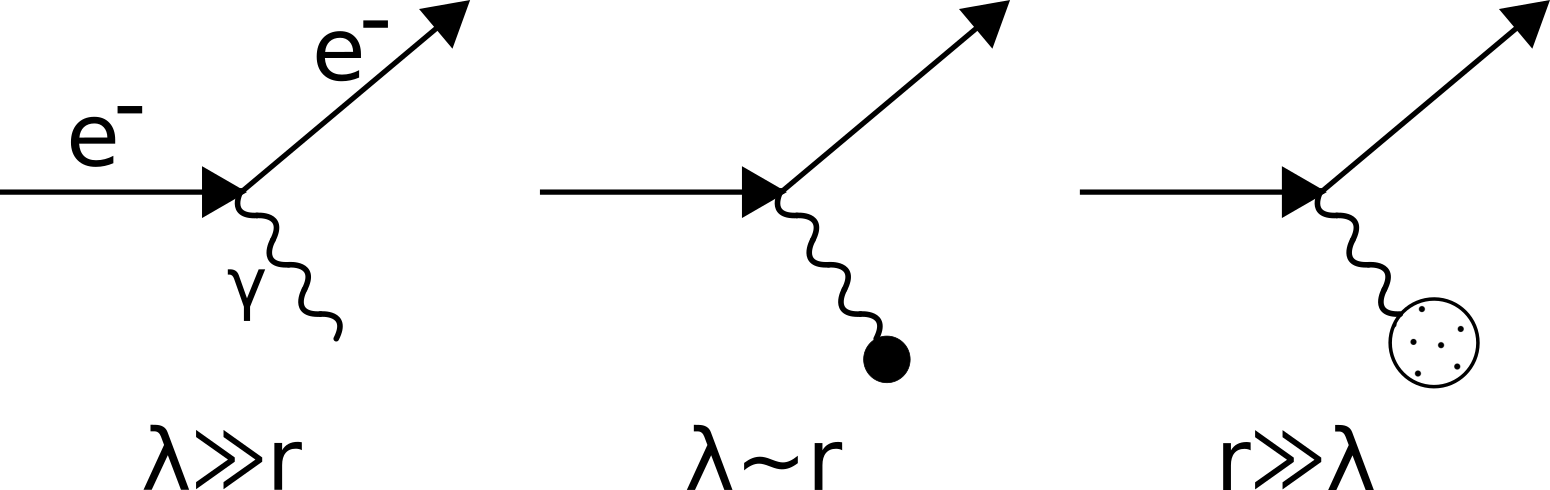
\includegraphics[width=280pt]{fig8_01}
\caption{Diagrammi di Feynman di un interazione elettrone nucleone}
\end{figure}

Come si può notare la reazione descritta con i diagrammi di Feynman avviene attraverso un fotone virtuale. 
L'elettrone, dopo lo scontro viene scatterato.
Come evidenziato in figura la relazione tra la lunghezza d'onda e il raggio del bersaglio determina la quantità di dettagli rilevabili.
L'ultimo diagramma riferito al caso in cui la lunghezza d'onda è molto minore del raggio del protone verrà studiata più avanti e corrisponde al caso di scontro profondamente inelastico (è il caso che rivela la struttura del nucleone). 
Ci concentreremo per ora sui primi due casi corrispondenti ad urti elastici.

%nuova sezione--------------------------------------------------------
\subsection{Diffusione elastica elettrone protone}
Il punto di partenza di tutta la trattazione è stata la \emph{sezione d'urto di Rutherford} in cui era considerata esclusivamente l'interazione coulombiana e sia  sonda che bersaglio erano approssimato puntiformi.

Si è poi passati alla sezione d'urto di Mott con cui si è in grado di studiare la struttura nucleare, le ipotesi in questo caso sono il bersaglio puntiforme e privo di spin e la sonda composta da elettroni relativistici con spin.
Nell'approssimazione di avere elettroni esclusivamente relativistici ($\beta=v/c\to 1$) la sezione d'urto di Mott corrisponde a
\begin{equation}
\left(\frac{d\sigma}{d\Omega}\right)_{Mott}^*=\left(\frac{d\sigma}{d\Omega}\right)_{Ruth}\cos^2 \frac{\theta}{2}
\end{equation}
L'asterisco indica il fatto che non viene considerato il rinculo del nucleo, questa è una buona approssimazione nel caso di basse energie ma non può essere sempre valido.

\paragraph{Rinculo del bersaglio}
Consideriamo il caso in cui il rinculo del bersaglio sia rilevante.
Si prende una sonda (elettrone) e un bersaglio (protone) di massa $m_e, M_p$ e caratterizzati inizialmente dai quadrivettori
\begin{equation}
p=\left(\frac{E}{c}, \vec{p}\right)\hspace{1cm}P=(M_pc, 0)
\end{equation}
E dopo l'urto da
\begin{equation}
p'=\left(\frac{E'}{c}, \vec{p'}\right)\hspace{1cm} P=\left(\frac{E_p}{c}, \vec{P'}\right)
\end{equation}
\begin{figure}[h]
\centering
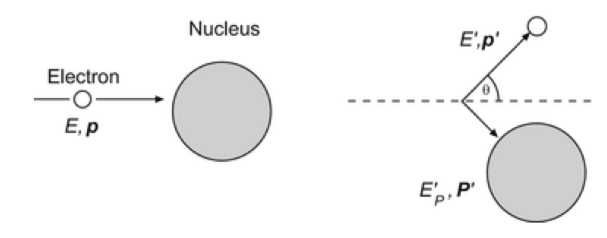
\includegraphics[width=200pt]{fig8_02}
\end{figure}

Per la conservazione del quadrivettore energia impulso si ottiene
\begin{equation}
p+P =p'+P'
\label{D:1.2}
\end{equation}
di cui posso fare il quadrato
\begin{equation}
p^2+2p\cdot P+P^2 =p'^2+2p'\cdot P'+P'^2
\label{D:1.1}
\end{equation}
Siccome la diffusione è elastica, la massa invariante dell'elettrone e del protone (non soggetta ad effetto relativistico) restano invariate.
\begin{equation}
p^2=p'^2=m_e^2c^2\hspace{1cm}P^2=P'^2=M_p^2c^2
\end{equation}
Sostituendo nella formula ~\eqref{D:1.1}, ottengo 
\begin{equation}
p\cdot P=p'\cdot P'
\end{equation}
Dove $P'$ può essere ricavato dalla formula ~\eqref{D:1.2}
\begin{equation}
p\cdot P =p'\cdot (p+P-p')=p'p+p'P-m_e^2c^2
\end{equation}
Esplicitiamo le relazioni e moltiplichiamo per $c^2$
\begin{equation}
E\cdot M_pc^2=E'E-\vec{p}\cdot \vec{p'}c^2+E'M_pc^2-m_e^2c^4
\end{equation}
Considerando la condizione di alte energie $E>m_ec^2$ posso considerare nulla la massa dell'elettrone, sostituendo poi al prodotto scalare il coseno e considerando che in condizioni relativistiche $E=pc$ si ottiene
\begin{equation}
E\cdot M_pc^2=E'E(1-\cos\theta)+E'Mc^2
\end{equation}
Si trova infine la relazione tra l'energia dell'elettrone diffuso e quello incidente.
\begin{equation}
E'=\frac{E}{1+\frac{E}{M_pc^2}(1-\cos\theta)}
\end{equation}
La questione importante è che c'è una relazione univoca tra l'energia dell'elettrone diffuso e l'angolo di diffusione.

Questa trattazione sarebbe la stessa se al posto di un protone si mettesse un nucleo.
Osservando quindi il grafico dell'energia in funzione dell'angolo di diffusione si può notare come per bersagli pesanti (nuclei) e elettroni a energia più bassa l'approssimazione di assenza di rinculo resti valida restituendo elettroni ad energia sempre costante a qualsiasi angolo.
Ma nel momento in cui si va a vedere il caso del bersaglio protonico o si aumenta notevolmente l'energia della sonda gli elettroni diffusi iniziano a cedere una parte di energia non trascurabile al nucleo.
\begin{figure}[h]
\centering
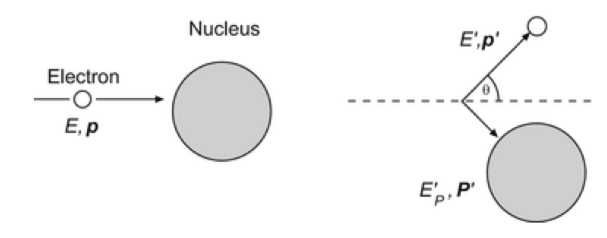
\includegraphics[width=200pt]{fig8_02}
\end{figure}

La sezione d'urto di Mott in questo caso varierà rispetto a quella vista fin'ora e deve essere moltiplicata di un ulteriore fattore
\begin{equation}
\left(\frac{d\sigma}{d\Omega}\right)_{Mott}=\left(\frac{d\sigma}{d\Omega}\right)_{Mott}^*\frac{E'}{E}
\end{equation}
Nelle considerazioni che dobbiamo fare esiste un altro parametro importante che è il momento trasferito
\begin{equation}
q^2=(p'-p)^2=\frac{4E'E}{c^2}\sin^2\frac{\theta}{2}
\label{D:1.3}
\end{equation}
(non viene ricavato ma si può ricavare della formule sopra)
Spesso ci si riferisce alla formula ~\eqref{D:1.3} anche come $-Q^2$ in quanto così diventa una quantità positiva ed è più comoda nelle trattazioni.

\paragraph{Interazione di spin}
Dobbiamo rilasciare ora un'altra approssimazione fatta precedentemente,infatti tra elettroni e protoni può esservi interazione di spin.
Il momento magnetico di una particella legato allo spin è
\begin{equation}
\mu =g\frac{e}{2M}\frac{\hbar}{2}
\end{equation}
Dove $g$ è detta \emph{anomalia magnetica} ed è ciò che distingue tra  un sistema classico e uno quantistico.
Il $g$ deriva dal fatto che la relazione tra momento angolare e momento magnetico valida nel caso classico, non vale per il momento magnetico di spin per cui è necessario introdurre appunto questo fattore.
Abbiamo visto che nel caso di particelle di Dirac prive di struttura interna questo fattore ha valore $g=2$.

Cerchiamo quindi di trovare la sezione d'urto per collisioni tra una sonda che è una particella ideale di Dirac e un bersaglio che è una particella ideale di Dirac, ossia tra particelle puntiformi con spin pari ad $1/2$.
Una parte dell'interazione dovrà essere magnetica e dovuta allo spin.
Dobbiamo considerare possibili eventi di spin flip (unico tipo di interazione possibile nel caso dello spin), la cui impossibilità era proprio alla base della sezione d'urto di Mott.

In questo caso viene inibita la diffusione a $0^o$, per lo stesso motivo per cui era inibito il back scattering nel caso di Mott, viene invece favorita la diffusione a $180^o$.
Vi è quindi l'introduzione di un termine di $\sin^2(\theta/2)$ nella sezione d'urto.
La sezione d'urto di particelle puntiformi a spin $1/2$ sarà quindi 
\begin{equation}
\left(\frac{d\sigma}{d\Omega}\right)_{S=\frac{1}{2}}=\left(\frac{d\sigma}{d\Omega} \right)_{Mott}\left(1+2\tau \tan^2 \frac{\theta}{2}\right)
\end{equation}
dove 
\begin{equation}
\tau=\frac{Q^2}{4M^2c^2}
\end{equation}
Che significato ha questo termine?
\begin{equation}
\begin{split}
\tau &\propto \mu \propto\frac{1}{M}\\
\tau &\propto Q
\end{split}
\end{equation}
Come si vede il termine è proporzionale sia al momento  di dipolo magnetico ( a sua volta proporzionale all'inverso della massa) che alla durata dell'interazione, infatti maggiore è la durata dell'interazione maggiore è la quantità di moto trasferita.

Ora quella che abbiamo trovato è l'interazione di particelle puntiformi ma come sappiamo il protone non è una particella puntiforme priva di struttura (non è quindi una particella fondamentale) e quindi dobbiamo generalizzare ancora queste formule per trovare la sezione d'urto adeguata.
Per tenere conto del fatto che il protone non è puntiforme si introducono i fattori di forma.
In particolare la sezione d'urto viene determinata dalla \emph{formula di Rosenbluth}
\begin{equation}
\left(\frac{d\sigma}{d\Omega}\right)=\left(\frac{d\sigma}{d\Omega}\right)_{Mott}\biggl[ \frac{G_E(Q^2)+\tau G_M(Q^2)}{1+\tau}+2\tau G_M(Q^2)\tan^2\frac{\theta}{2}\biggl]
\label{D:1.4}
\end{equation}
dove $G_E(Q^2)$ è il \emph{fattore di forma elettrico} e $G_M(Q^2$ è il \emph{fattore di forma magnetico}.

Questi fattori sono due funzioni che parametrizzano la nostra non conoscenza rispettivamente di distribuzione di carica e distribuzione di corrente all'interno del protone.
Sono delle grandezze che dobbiamo determinare sperimentalmente.
Si capisce che questa espressione parametrizza già la fenomenologia dell'interazione infatti abbiamo tra parentesi un primo termine che dipende da entrambi i fattori e un secondo termine che invece dipende esclusivamente dall'interazione magnetica.
In particolare i fattori di forma hanno un significato fisico nell'ipotesi in cui si studia $Q^2\to 0$ ovvero quando si ha una lunghezza d'onda del fotone virtuale (di momento trasferito) molto maggiore del raggio del bersaglio.
In pratica $Q^2\to 0$ si ha quando si osservano le proprietà globali ovvero quando non si va a perturbare il sistema con una sonda ma si è in un caso statico del bersaglio.
In questo limite si dovrà avere che il fattore di forma elettrico fa ricavare la carica del protone e il fattore di forma magnetico mi da il momento magnetico del protone.
\begin{equation}
\begin{split}
Q^2\to 0\hspace{1cm}&\frac{G^p_E}{e}\to 1\\
&\frac{G^P_M}{\mu}\to 2,79
\end{split}
\end{equation}
I dati sopra sono quelli quelli del protone ma essendo la formula universale devono valere anche nel caso del neutrone
\begin{equation}
\begin{split}
Q^2\to 0\hspace{1cm}&\frac{G_E^n}{e}\to 0\\
&\frac{G_M^n}{\mu}\to -1,91
\end{split}
\end{equation}

\paragraph{Misura sperimentale dei fattori di forma}
Abbiamo determinato la struttura teorica che sostiene questa teoria, ora ci mancano i dati sperimentali.
Per misurare sperimentalmente i fattori di forma devo pormi nella condizione di avere $Q^2$ costante e devo quindi studiare la formula di Rosenbluth.
Stando a $Q^2$ costante si può parametrizzare ~\eqref{D:1.4}
\begin{equation}
\frac{\left(\frac{d\sigma}{d\Omega}\right)_{Ros}}{\left(\frac{d\sigma}{d\Omega}\right)_{Mott}}=A(Q^2)+B(Q^2)\tan^2\frac{\theta}{2}
\end{equation}
Cosa rappresentando dunque $A$ e $B$?

Facendo il grafico della sezione d'urto in funzione della $\tan^2\frac{\theta}{2}$ quello che si ottiene è una retta con intercetta data da $A$ e pendenza da $B$.
\begin{figure}[h]
\centering
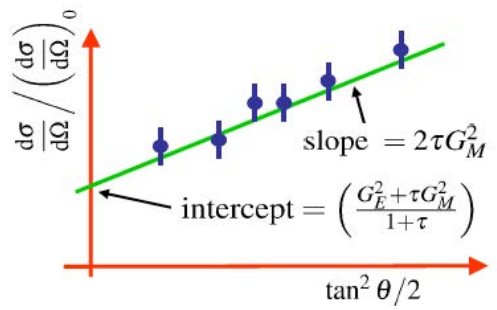
\includegraphics[width=150pt]{fig8_04}
\end{figure}
 
Siccome $\tau$ ha una dipendenza diretta da $Q^2$ e il fattore di forma magnetico è sempre moltiplicato per $\tau$ si ottiene che 
\begin{equation}
\begin{split}
Q^2\to 0
\hspace{1cm}
& \frac{\left(\frac{d\sigma}{d\Omega}\right)_{Ros}}{\left(\frac{d\sigma}{d\Omega}\right)_{Mott}}\to G^2_E(Q^2)\\
Q^2\to \infty
\hspace{1cm}
& \frac{\left(\frac{d\sigma}{d\Omega}\right)_{Ros}}{\left(\frac{d\sigma}{d\Omega}\right)_{Mott}}\to (1+2\tau\tan^2(\theta/2))G^2_M(Q^2)
\end{split}
\end{equation} 

%nuova sezione------------------------------------------------------
\subsection{Diffusione profondamente inelastica}
Viene più comunemente denominata \emph{Deep inelastic scattering} (DIS), in quanto è di uso comune la denominazione internazionale.
Come per la diffusione elastica anche in questa interazione si sfruttano gli elettroni.
La sezione d'urto completa per un urto elastico, nell'approssimazione $Q^2=-q^2\to \infty$, abbiamo visto che è
\begin{equation}
\left(\frac{d\sigma}{d\Omega}\right)_{Ros}=\frac{\alpha^2}{4E^2\sin^4\frac{\theta}{2}}\frac{E'}{E}\biggl[\frac{Q^2}{2M^2}G_M^2\tan^2\frac{\theta}{2}\biggl]
\end{equation}
Dove 
\[
G_M(Q^2)\approx \frac{1}{\left(1+\frac{Q^2}{0,71GeV^2}\right)^2}
\]
Facendo un grafico della sezione d'urto in funzione del $Q^2$ evidenzia una rapida decrescita all'aumentare di $Q^2$ con un andamento che rispecchia un fattore del tipo $Q^{-6}$.
Ci si aspetta quindi che la sezione d'urto vada molto rapidamente a $0$.
Questa sezione d'urto sarebbe quella che si si aspetterebbe se la materia all'interno del protone fosse distribuita in modo uniforme.

Negli anni '70 sono stati fatti esperimenti sulla materia all'interno del protone e questo era esattamente ciò che ci sia aspettava e le dinamiche che si sono verificate sono simili a quelle successe a Rutherford.
Quello che si è verificato sperimentalmente è che andando ad elevati $Q^2$ ci verifica quella che può essere vista come una collisione con delle particelle puntiformi.

\paragraph{Deep inelastic scattering}
Il fatto che la collisione sia inelastica comporta a non avere più una relazione univoca tra l'energia dell'elettrone diffuso $e'$ e l'angolo di diffusione $\theta$.
Si ha quindi che anche a stessi angoli è possibile trovare particelle con energia diversa.
Questo accade perché una parte dell'energia viene usata per eccitare il protone, per cui la massa del protone varia.
Questo effetto si può rappresentare con un digramma di Feynman del tipo mostrato in figura.
\begin{figure}[h]
\centering
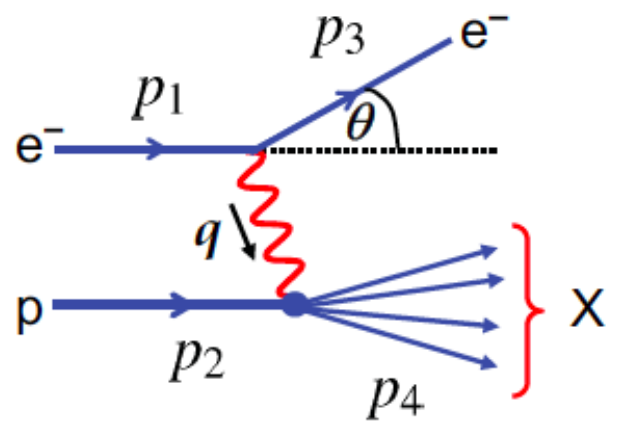
\includegraphics[width=150pt]{fig8_05}
\end{figure}

Come si può vedere il protone, rappresentato dal quadrivettore $p_2$, dopo l'interazione diventa una serie di prodotti d'interazione il cui insieme viene indicato con $X$.
Il quadrivettore di questi prodotti dell'interazione lo caratterizziamo come $p_4$.

Ciò che stiamo facendo ora è cercare di caratterizzare le variabili cinematiche addizionali che permettono di determinare il processo.
In particolare
\begin{equation}
Q^2=-q^2=(p_3-p_1)^2
\end{equation}
mentre la massa invariante corrisponde a 
\begin{equation}
M^2_x=p_4^2=(q+p_2)^2=-Q^2+2p_2\cdot q+M_p^2
\end{equation}
Per caratterizzare l'inelasticità del processo bisogna calcolare la relazione tra la massa invariante prima dello scontro rispetto a quella dopo lo scontro.
Questa quantità è definita \emph{$X$ di Bjorken} e corrisponde a 
\begin{equation}
X=\frac{Q^2}{2p_2\cdot q}
\end{equation}
\'E una grandezza significativa perché calcolando
\begin{equation}
Q^2=2p_2\cdot q+M_p^2-M_x^2
\end{equation}
si può vedere che nel caso di un processo elastico la differenza $M_p^2-M_x^2$ è pari a $0$ ma invece nel caso del processo inelastico corrisponde proprio alla $X$ di Bjorken.
In particolare si può vedere che il processo è elastico se $X=1$ mentre è inelastico se $X<1$.
Questa è una variabile importante perché non caratterizza semplicemente la cinematica della reazione ma ha un significato fisico in quanto caratterizza i componenti puntiformi del protone.

Le variabili che caratterizzano un processo inelastico sono quindi
\begin{equation}
Q^2\hspace{1cm} X
\end{equation}
a cui va aggiunta un variabile ulteriore che viene usata alle volte
\begin{equation}
\nu=E_1-E_3
\end{equation}
che è l'energia trasferita dall'elettrone al bersaglio.
Solitamente si utilizzano solo due di queste variabili a seconda delle situazioni in quanto bastano per descrivere un processo di interazione inelastica.

Siamo ora in grado di comprendere questo tipo di sperimentazione, il tipo di configurazione sperimentale è la stessa del processo di interazione inelastico, tanto che furono usati gli stessi acceleratori.
Nella prima generazione di esperimenti ciò che si contava erano esclusivamente gli elettroni diffusi mentre poi è stato possibile rilevare anche i prodotti di interazione.
Di fatto ci si poneva ad un certo angolo e si misurava l'energia dell'elettrone diffuso potendo così arrivare a ricavare la sezione d'urto.
La sezione d'urto in questo caso era in due variabili.
Nel grafico sotto viene mostrata questa sezione d'urto in funzione dell'energia dell'elettrone diffuso
\begin{figure}[h]
\centering
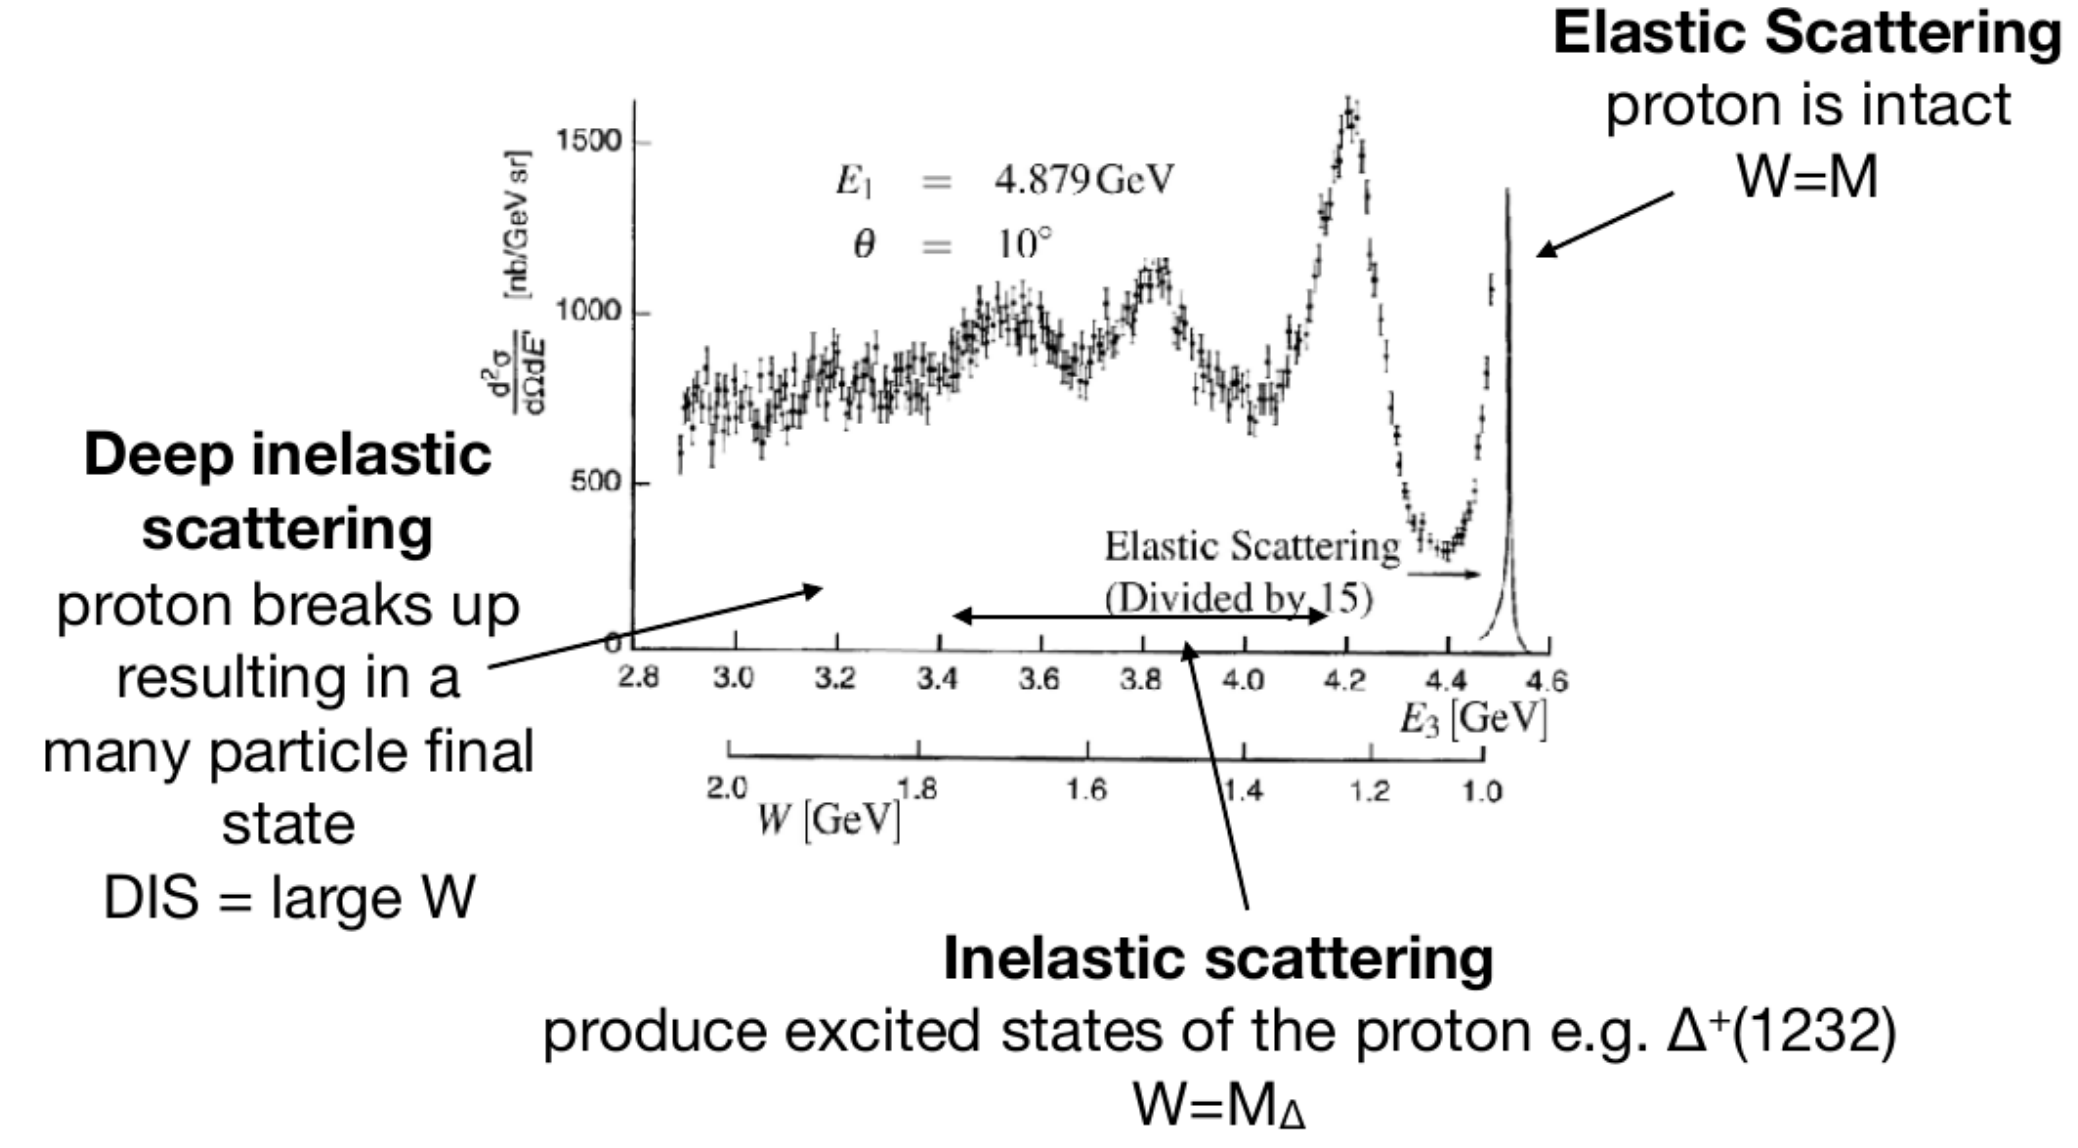
\includegraphics[width=200pt]{fig8_06}
\caption{Sezione d'urto differenziale di interazione inelastica in funzione dell'energia $E_3$ dell'elettrone diffuso}
\end{figure}

La zona indicata in figura come la zona di scattering inelastico è detta anche \emph{zona delle risonanze} e comprende i vari stati eccitati del protone come per esempio il $\Delta^+(1232)$, questa particella ha la stessa configurazione del protone (due quark up e uno down) ma invece di avere spin $s=1/2$ ha spin $s=3/2$ (tutti i quark hanno spin allineato in questo caso).
Questo stato del protone è da considerarsi proprio come una particella diversa, infatti la differenza di massa è notevole (1232 contro i 938 classici).
Spostandosi poi verso le zone a energia $E_3$ minore (che ci indica un'energia di massa maggiore in quanto l'energia persa dall'elettrone deve necessariamente essere passata al protone ) si verifica un appiattimento della curva con la sezione d'urto che diventa costante, ci si trova quindi nella zona di interazione profondamente inelastica.
Ricordando la trattazione iniziale in questa zona era previsto un annullamento della sezione d'urto (all'aumentare di $Q^2$ la sezione d'urto si annullava), ma i dati sperimentali smentiscono questo andamento.
Il fatto che questo annullamento non ci sia indica che la distribuzione di massa all'interno del protone non può essere uniforme ma presenta delle concentrazioni puntiformi (questo perché la distribuzione è piatta ma sfruttando l'interpretazione con le trasformate di Fourier per risalire alla funzione che le genera si può fare un'antitrasformata che nel caso di una distribuzione piatta coincide con la delta di Dirac, fisicamente rappresentabile da particelle puntiformi).
 
\paragraph{Sezione d'urto del DIP}
La sezione d'urto trovata per spiegare questa zona di \emph{Deep inelastic scattering} è un aggiornamento della sezione d'urto di Rosenbluth.
\begin{equation}
\frac{d^2\sigma}{d\Omega dE_3}=\left(\frac{d\sigma}{d\Omega}\right)_{Mott}\biggl[W_2(Q^2,\nu)+2W_1(Q^2,\nu)\tan^2\frac{\theta}{2}\biggl]
\end{equation}
Le funzioni $W_1, W_2$, non si chiamano più fattori di forma ma \emph{funzioni di struttura} e sono la grandezza sconosciuta che va ricavata sperimentalmente.
Solitamente rispetto a questo tipo di sezione d'urto si introducono altre due funzioni di struttura che introducono due quantità diverse e adimensionali; nei plot infatti non si usano le W ma queste altre due funzioni
\begin{equation}
\begin{split}
F_1(X, Q^2) & =M_c^2W_1(Q_1^2,\nu)\\
F_2(X, Q^2) & =\nu W_2(Q^2,\nu)
\end{split}
\end{equation} 
dove $F_1$ è una funzione puramente magnetica (analogamente al fattore di forma magnetico, mentre $F_2$ è una funzione mista e quindi elettromagnetica (come accadeva nella sezione d'urto di Rosenbluth).
Queste sono le grandezze che sono state misurate sperimentalmente.
\begin{figure}[h]
\centering
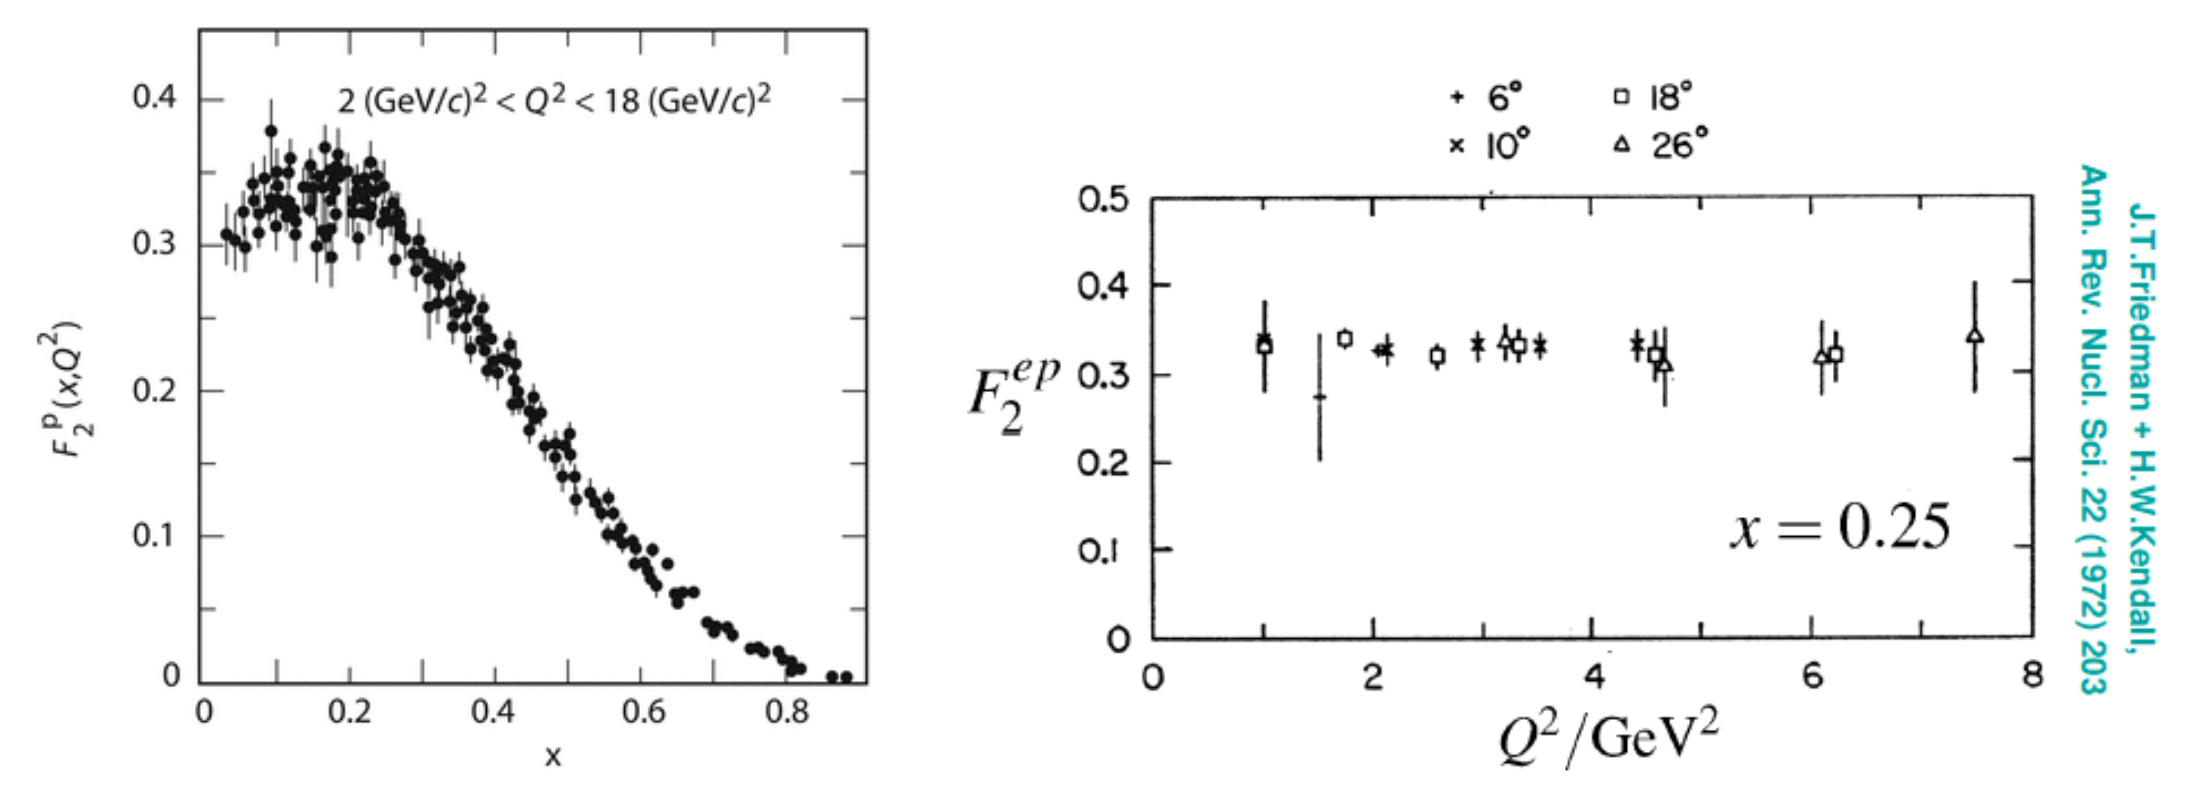
\includegraphics[width=250pt]{fig8_07}
\caption{Risultati sperimentali di $F_2$ in funzione a sinistra di $X$ e a destra di $Q^2$}
\label{D:5}
\end{figure}

I grafici in figura ~\ref{D:5} rappresentano l'andamento della funzione di struttura elettromagnetica in funzione della $X$ di Bjorken e della $Q^2$.
Da notare che la $F_2$ è costante in funzione di $Q^2$ il che vuol dire che non dipende dal momento trasferito.
$Q^2$ corrisponde alla lunghezza d'onda della sonda utilizzata, che come abbiamo visto precedentemente ci indica anche la risoluzione di analisi, quindi la $F_2$ è indipendente dalla risoluzione con cui si analizza il bersaglio.
Si può dire quindi che $F_2$ è una funzione scalabile, ovvero che l'interazione avviene con oggetti puntiformi (non siamo in grado di risolvere la struttura degli elementi con cui effettuiamo l'interazione).
Si ha che le funzioni di struttura possono essere riscritte come
\begin{equation}
F_1(Q^2, X)\to F_1(X)\hspace{1cm} F_2(Q^2, X)\to F_2(X)
\end{equation} 

Si è trovato poi che vi è una relazione diretta tra $F_1(X) $ e $F_2(X)$ rappresentata nel grafico sotto
\begin{figure}[h]
\centering
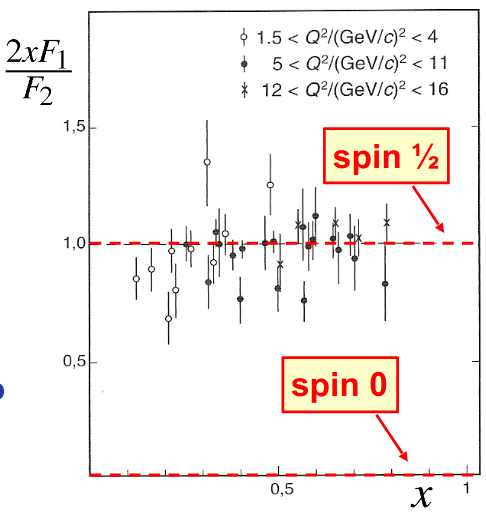
\includegraphics[width=150pt]{fig8_08}
\end{figure}

Questo rapporto ci indica che stiamo interagendo con particelle di spin $1/2$.
Se l'interazione avvenisse con oggetti di spin $0$ allora il rapporto tra le funzioni di struttura sarebbe $0$.
Questo deriva dalla dipendenza magnetica della sezione d'urto.

\paragraph{Modello a partoni/quark}
Introduciamo ora il modello a partoni ovvero un modello che comprende queste particelle subprotoniche puntiformi che poi potremo ricondurre a quelle che adesso sappiamo essere i quark.

Per comprendere meglio il tipo di interazione ciò che è stato necessario fare è di prendere il diagramma di Feynman e ampliarne il significato rivedendo il tipo di interazione.
Quello che è stato fatto è, piuttosto che considerare l'interazione con il protone che poi si divide, di considerare il protone come un insieme di componenti che andranno ad interagire singolarmente con la sonda.
\begin{figure}[h]
\centering
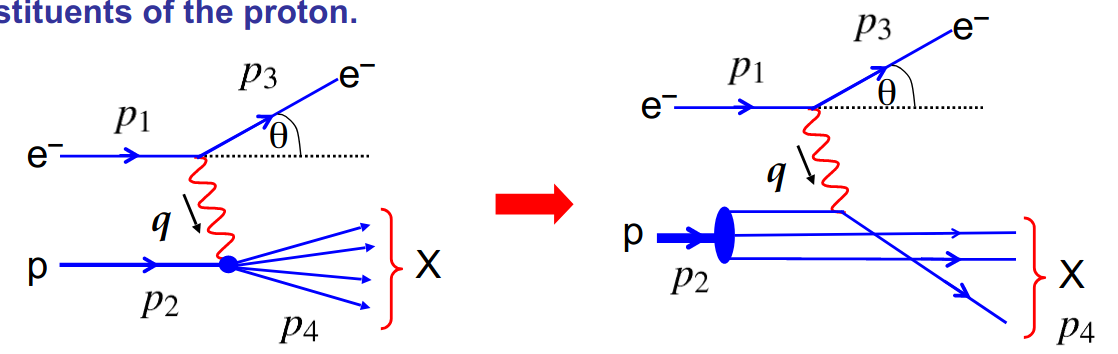
\includegraphics[width=200pt]{fig8_09}
\end{figure}

Questo tipo di significato fisico è solitamente rappresentato da quello che si chiama \emph{infinite momentum frame}.
Ci mettiamo in un sistema di riferimento in cui trascuriamo i gradi di libertà trasversi assumendo in pratica che il protone abbia una tale quantità di moto longitudinale da poter trascurare le sue componenti trasversali.
In questo modo l'unica grandezza che mi deve interessare è la quantità di moto nella direzione dell'interazione.
In questa approssimazione assumiamo che il protone abbia un quadrivettore del tipo
\begin{equation}
(E_2,\vec{p_2})
\end{equation}
E che le componenti del protone abbiamo una frazione della sua quantità di moto (e di conseguenza del suo quadrivettore
\begin{equation}
(\eta E_2, \eta \vec{p_2})
\end{equation}
L'interazione può venire rappresentata come in figura
\begin{figure}
\centering
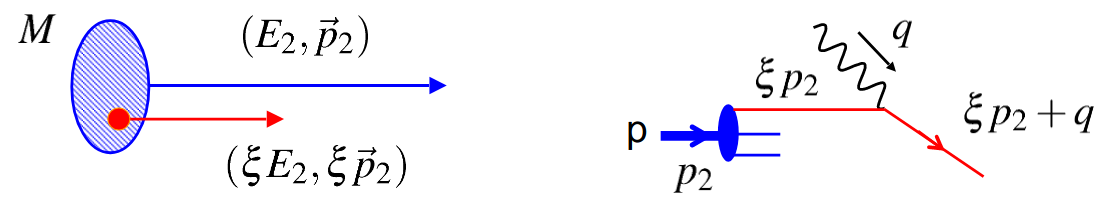
\includegraphics[width=200pt]{fig8_10}
\end{figure}

Si ha
\begin{equation}
(\eta p_2+q)^2=mq^2
\end{equation}
dove $m$ è la massa invariante di questi componenti del protone e possiamo considerare tendente a $0$.
\begin{equation}
\eta^2p_2^2+2\eta p_2q+q^2-mq^2=0
\end{equation}
$\eta^2 p_2^2=mq^2$ in quanto è il modulo quadro del momento prima dell'interazione.
Quello che rimane è 
\begin{equation}
q^2+\eta p_2q=0
\end{equation}
La variabile $\eta$ è la frazione di quantità di moto del protone portata dal partone (ovvero la particella componente del protone) e corrisponde a
\begin{equation}
\eta=\frac{-q^2}{2p_2q}=\frac{Q^2}{2p_2q}=X
\end{equation}
Si vede che il significato fisico della $X$ di Bjorken che abbiamo introdotto precedentemente come \emph{inelasticità del processo} è interpretabile in questo modello a partoni come la frazione di quantità di moto portata dal singolo partone.
In questo caso ciò mi fa avere un'interpretazione importante delle funzioni di struttura che erano precedentemente delle quantità introdotte semplicemente per parametrizzare l'ignoranza che c'era sulla struttura del protone.
In realtà in questo caso di può dire che la diffusione profondamente inelastica può essere interpretata come la diffusione elastica su particelle puntiformi di spin $s=1/2$ che costituiscono il protone.

Con questo tipo di interpretazione, la $X$ di Bjorken ha un significato fisico ben preciso e quindi la sezione d'urto, che prima avevamo ricavato solo da un punto di vista fenomenologico, ora può essere rivista.
Innanzitutto si ha che stiamo agendo su particelle cariche.
La sezione d'urto elementare è dunque proporzionale alla carica delle particelle al quadrato, non conoscendo però la carica di quese particelle è necessario introdurre un fattore $Z_f$.
\begin{equation}
\frac{d\sigma}{d\Omega}\propto (Z_f\cdot e)^2
\end{equation}
dove $Z_f\cdot e$ è la carica dei componenti del protone.

A questo punto devo caratterizzare queste distribuzioni.
Identifico come 
\[
q_f(x)
\]
la distribuzione di impulso dei quark di tipo $f$ e come
\[
\bar{q}_f(x)
\]
la distribuzione di antiquark di $f$.
La relazione che lega materia e antimateria è il fatto di avere massa uguale e spin uguale ma carica di segno opposto si differenziano esclusivamente per la carica).
\'E ragionevole pensare che analogamente al caso elettrone-positrone possa esserci una coppia del tipo quark e antiquark.
Con questo tipo di assunzione posso supporre che quello che abbiamo definito come scattering inelastico sia in realtà uno scattering elastico su questo tipo di particella, ossia sui quark/partoni.
Abbiamo visto inoltre che i quark sono caratterizzati da un unica quantità che corrisponde alla frazione di quantità di moto del protone che portano.
Introduciamo quindi una funzione $F_2(X)$ che non è più un artificio sperimentale ma mi restituisce esattamente la quantità di moto dei quark.
\begin{equation}
F_2(X)=X\sum_f Z_f^2(q_f(X)+\bar{q}_f(X))
\end{equation}
In questo modo è possibile trovare una sezione d'urto per questo tipo di interazione.
La sezione d'urto totale di deep inelastic scattering può essere ottenuta come somma incoerente di interazione con i singoli quark all'interno del protone.

\paragraph{Funzione di struttura $F_2$}
Studiamo quindi la funzione $F_2$.
\begin{figure}
\centering
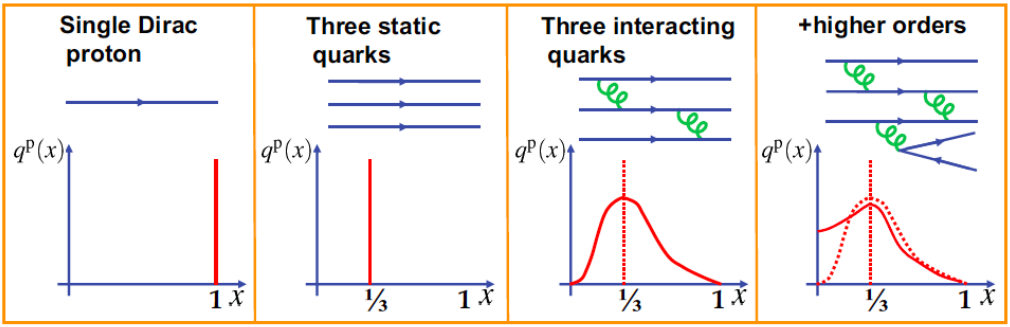
\includegraphics[width=\columnwidth]{fig8_11}
\end{figure}

I grafici sopra mostrano lo studio della distribuzione $q(X)$, corrispondente alla distribuzione che hanno i partoni con una certa quantità di moto $X$, in funzione di $X$.
Sono quattro grafici differenti in quanto danno uno spaccato dell'andamento della distribuzioni con delle ipotesi differenti

\begin{itemize}
\item Nel primo grafico a sinistra si è supposto che il protone fosse composto da un unica particella.
In questo caso la distribuzione è composta da un unico picco su $X=1$, in quanto tutta la quantità di moto sarebbe portata da questo unico partone.

\item Il secondo grafico rappresenta il caso in cui ci sono tre partoni che non interagiscono a comporre il nucleo.
Anche qui si trova un picco ma posizionato a $X=1/3$ in quanto ogni partone ha un contributo identico e fisso.

\item Le cose diventano più interessanti nel terzo caso di tre partoni differenti ma interagenti tra di loro.
Ciò che ci si può aspettare è quindi una funzione non più piccata ma estesa e con una media a $1/3$.
Questo descrive il fatto di poter scambiare quantità di moto tra le tre particelle.
La funzione si azzererà nei punti $X=0$ e $X=1$.

\item L'ultimo grafico, che è quello che poi si è visto sperimentalmente, rappresenta una curva del tutto simile a quella precedente ma con la differenza che in $X\to 0$ questa non va a $0$.
Ciò vuol dire che non solo i partoni interagiscono tra di loro ma che nella loro interazione possono portare alla generazione di altre particelle.
Effettivamente un gluone che viene scambiato può dare luogo ad una coppia $q, \bar{q}$.
In pratica il protone non è un oggetto fisso ma è un continuo ribollire di particelle che si generano e ritornano nel vuoto, soddisfacendo il principio di indeterminazione di Heisenberg.
Una particella di massa infinita può durare per un tempo infinitesimo non violando il principio di indeterminazione.
$X\to 0$ vuol dire in pratica una ripartizione infinitesima della quantità di moto.

Altra cosa interessante è che facendo un integrale di questa funzione, essendo una distribuzione dovrebbe restituire $1$ ma si è visto sperimentalmente che questo integrale da come risultato $1/2$.
Significa quindi che i quark contribuiscono solo al $50\%$ della quantità di moto del protone, l'altra metà è portata dai gluoni.
Non riusciamo a vedere i gluoni in quanto evidentemente questi non interagiscono con gli elettroni in quanto questo possono interagire solo con particelle cariche.
\end{itemize}

\paragraph{DIP semi-inclusivo}
Quello di cui abbiamo parlato fino a qui era il deep inelastic scattering inclusivo ovvero che prevede la rivelazione esclusivamente degli elettroni.
Negli esperimenti della generazione successiva si parla invece di \emph{DIP semi-inclusivo}, in cui non viene rivelato solamente l'elettrone ma anche i prodotti della reazione e in particolare se la reazione avviene con un quark $up$ questo sarà sparato fuori dalla particella.
Una delle peculiarità della forza forte è che i singoli quark non sono mai stati visti.
La forza forte è molto diversa dalle altre, è una forza che possiede una peculiarità che si chiama \emph{libertà asintotica}, che prevede che se le particelle sono a contatto la forza è nulla ma che aumenta linearmente con la distanza.
Quindi più le particelle sono distanti e più aumenta la forza, per cui se si cerca di estrarre un quark da un protone l'energia di interazione è tale da creare un ulteriore particella.

Per esempio estraendo un quark $up$ su ha questo interagisce con un quark $\bar{d}$ generando una particella detta $\pi^+$ (mesone positivo).
Se riesco a rivelare questo mesone positivo so che l'interazione è stata con un quark $up$.
Allo stesso modo i quark $down$ generano $\pi^-$ (mesoni negativi).
Riuscendo a rivelare queste particelle possiamo quindi approfondire la nostra conoscenza sull'interazione.


